%%% Local Variables: 
%%% mode: latex
%%% TeX-master: "../KanjiHWR"
%%% End: 

\chapter{Japanese Script}
\label{sec:japansescript}

The Japanese writing system has a long history. It goes back to around 800 A.D. 
The Japanese script is in fact a writing system, as Japanese is denoted in 
a combination of three different scripts: \emph{Hiragana}, \emph{Katakana} and 
\emph{Kanji}. Kanji is a conceptual script, where each character bears the 
meaning of one or more semantic concepts and represents morphemes. 
Hiragana and Katakana are both syllabic scripts, and the individual characters do
not bear reference to concepts or even words, but merely to phonological units, 
usually two phonemes.

In this chapter, the development of the script will be reviewed in 
section~\ref{sec:ashorthistoryofjapanesewritingsystem}.
In section~\ref{sec:modernjapanesewritingsystem} the current Japanese writing 
system will be exemplified, with a focus on the Kanji in 
section~\ref{sec:compositionofkanji}. Hiragana and Katakana will be reviewed in
section~\ref{sec:kana}, which centers around the Kana scripts. 
Machine processing of the different Japanese scripts and the difficulties that
go along will be demonstrated in section~\ref{sec:machinewritingofjapanese}.
The difficulties of learning to use the Japanese script will be illustrated in 
section~\ref{sec:writingjapanesedifficulties}.

\section{A Short History of the Japanese Script}
\label{sec:ashorthistoryofjapanesewritingsystem}

The historical development of the Japanese script is tightly connected to the 
history of the Kanji characters. Kanji, in Japanese 
\cjk{漢字}~(Jap. pron. \cjk{カンジ} / kanji; Eng.~lit.~\emph{Han~characters}) 
refers to the 'characters of the Han', meaning the Han Dynasty 
(206 B.C.-220 A.D.; simplified Chinese: \cjk{汉朝}; traditional Chinese: 
\cjk{漢朝}) \shortcite{Foljanty1984}. In Mandarin the same characters are 
referred to as \emph{Hànzì} (simplified Chinese: \cjk{汉字}; 
trad. Chinese: \cjk{漢字}).
Note, that the first character \cjk{漢} (Chin. 'han', Jap. 'kan', Eng. 'Han') 
of both the words \emph{Han dynasty} and \emph{Kanji} is identical in Japanese 
and traditional Chinese, even though it has a different pronunciation in the 
Chinese and Japanese language. In traditional Chinese the character with
the same meaning (\cjk{汉}) has a different shape. This apparent oddity will be 
explained in greater detail in 
section~\ref{sec:historicaldevelopmentofjapanesescript}.

\subsection{Historical Development}
\label{sec:historicaldevelopmentofjapanesescript}
%xxx: see \shortcite{Foljanty1984} 2.1.1-2.1.3
%xxx: see wikipedia article
%xxx: see \shortcite{Grassmuck1997}
%xxx: see \shortcite{Chamberlain1982} for the Kojiki

\subsubsection{History of the Kanji}
\label{sec:historyofthekanji}

The Kanji script as developed and coined by the Han is in principle still valid 
today. It is used alone or in combination with phonetic spelling in China, Japan,
Taiwan, Hongkong. In Vietnam it was used before it was replaced with the 
Vietnamese alphabet (Viet.: 'quốc ngữ', Eng. lit. 'national language', Eng. 
'national script'), a script based on the Latin alphabet. In South Korea the Han 
characters were in use until they were replaced with 
Hangul~(Kor. with Han characters \cjk{韓國語}; Eng. 'Korean')~\shortcite{Foljanty1984}.

The Kanji characters were brought to Japan by Koreans living in Japan around 
300-400 A.D. Since the Kanji were used by the Koreans to write 
Hangul they also used it to write Japanese. There was no other Japanese script 
before that time. Reports about an original Japanese script called 
\emph{Jindai Moji} (Jap. \cjk{神代文字}; Eng. 'scripts of the age of the gods')
could not be proven. They are now assumed to be a political and speculative 
invention by Japanese Nationalists in the early 
19th.~century~\shortcite{Foljanty1984}. According to \shortcite{Lange1922}
the \emph{Kogo Shūi} (Jap. 古語拾遺; a historical record of the Inbe clan),
which was written around 800 B.C. denies the presence of a Japanese native
script before the introduction of the Han characters. However, the questions
seems irrelevant in the sence, that no longer text or document has been found,
written in that script.

In the Christian year 712 an ancestral act of writing was performed at 
Japanese emperor Temmu's court. Hieda~no~Are, a member of the guild of the 
\emph{kataribe} or reciters, basically a Japanese Griot, dictates the 
\emph{Kojiki} (Jap. \cjk{古事記}; Eng. 'Record of Ancient Matters') to 
Ō~no~Yasumaro. Ō~no~Yasumaro wrote the Kojiki, which is not the first written 
document found in Japan, however it is Japan's oldest attempt to write down 
spoken Japanese~\shortcite{Grassmuck1997,Chamberlain1982}.

At the time the Han characters were first used to write Japanese, 
they were already a developed script, more than 1,000 years old, 
as they stabilised to their modern form within the Han 
period\footnote{Also see timeline in section~\ref{sec:app:kanjitimeline}.}~\shortcite{Grassmuck1997}.

The first chinese characters were found on oracle bones from the Shang Dynasty
(Chinese \cjk{商朝}), which ruled over China some 500 to 600 years within the 
time period between 1600 B.C. and 1046 B.C.~\shortcite{Grassmuck1997,Guo2000}.

According to the Kojiki, a scholar called Wani (Jap. \cjk{王仁}) from Korea 
brought two foundational Chinese books to Japan, the \emph{Lunyu} 
(Simplified Chin. \cjk{论语}; trad. Chinese: \cjk{論語}; Eng. 'Analects'), 
also known as \emph{The Analects of Confucius} and 
the \emph{Qianziwen} (Chin./Jap. \cjk{千字文}; Jap. 
pron.~\cjk{センジブン}/senjibun; Eng. 'The Thousand Character Classic'),
which is a Chinese poem used as a primer for teaching Chinese characters to 
children. It contains exactly one thousand unique 
characters~\shortcite{Grassmuck1997}. The Chinese language comprehends more 
than 40,000 Hànzì characters lexicographically. Only around 25\% of those 
including about 250 \emph{Kokuji} (Jap. \cjk{国字}; Eng. 'national characters') 
are in Japanese dictionaries. Only around 2,000-3,000 of those are part of the 
common characters~\shortcite{Foljanty1984}. 

The Japanese Ministry of Education issued a list of 1,850 standard Kanji in 1946
under the name of \emph{Tōyō kanjihyō} (Jap.~\cjk{当用漢字表};
Eng.~'list of Kanji for general use'). The list of Tōyō Kanji was slightly 
revised and extended in 1981 and comprised 1,945 Kanji as the Jōyō Kanji
(Jap. \cjk{常用漢字}; Eng. 'often used Kanji')~\shortcite{Foljanty1984}.
As of 2010 a revised list of 2,131 characters is in official 
use~\shortcite{Noguchi2009}. 

In China there had been a spelling reform in the 1950s, affecting many of the
general use characters, resulting in simplified Chinese. In Japan, the Ministry
of Education issued it's own reform when the Tōyō kanji list was introduced.
However, the Japanese reform affected a smaller set of characters of only a few 
hundred and resulted in Shinjitai (Jap. shinjitai: \cjk{新字体}; 
Jap. kyūjitai: \cjk{新字體};
Jap. pron. \cjk{シンジタイ}/shinjitai; Eng. 'new character form'), 
which replaced the Kyūjitai 
(Jap. shinjitai: \cjk{旧字体}; Jap. kyūjitai: \cjk{舊字體}; 
Jap. pron.~\cjk{キュウジタイ}/kyūjitai; Eng. lit. 'old character forms'). 
This explains how some characters are still identical in traditional Chinese and 
Japanese, because they were not affected by any spelling reform, like the 
afforementioned \cjk{漢} (Jap. pron. \cjk{カン}/kan; Chin. pron. 'hàn'),
while other characters are different, like the simplified 
Chinese 'hàn': \cjk{汉}. Henceforth, and throughout this document, all Japanese characters are in the new character form shinjitai.

\subsubsection{Typology of the Kanji}
\label{sec:typologyofthekanji}

In order to study the Kanji and their composition, it is useful to know how they
were first indendet and built. Integrated as the integral part into the Japanese
writing system, despite the reform and the choice different subsets of what is 
considered the standard character set, the characters are still mainly composed
the way as intendet by the scholars of the Han period.

From the religious writings on the oracle bones mentioned in 
section~\ref{sec:historicaldevelopmentofjapanesescript} a secular script 
emereged. In parallel, the process of graphical abstraction advanced and
finished around 100-200 A.D., leaving aside the modern reforms of the 
20th~century. The invention of the paint-brush around 100 B.C. improved and 
simplified writing, also the writing surfaces in their order of appearance,
bone, stone, metall, wood and then paper, brought further simplification and
spreading of writing. Paper and paint-brush offered the possibilty to write
without hindrance and technical coincidences, therefore it was possible to
standartise the characters and improve them from artistic and aesthetic 
viewpoints.

%xxx: Put some real Kanji pictograms here after Kano1990 lesson 1+2
\begin{figure}[htbp]
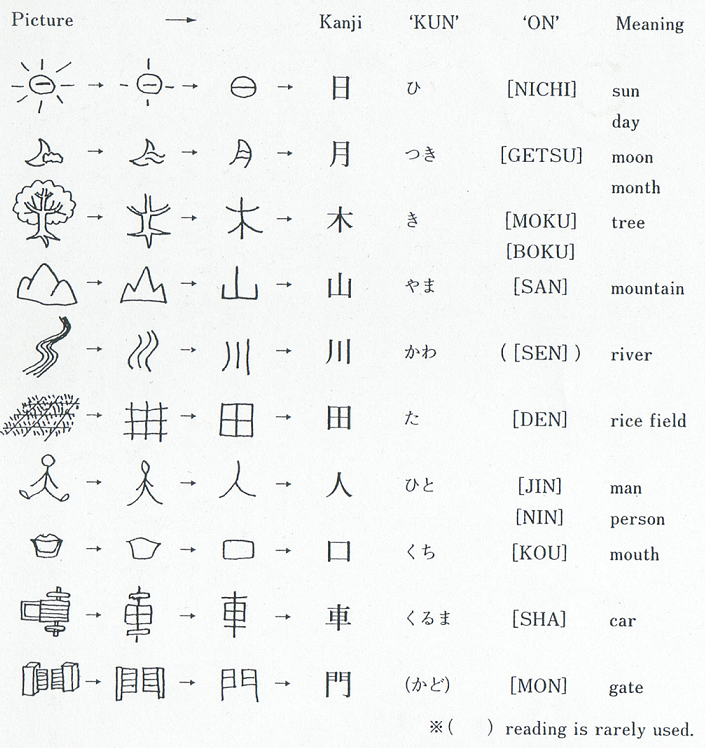
\includegraphics[scale=0.5]{images/kanjipictograms.png}
\caption{Kanji pictograms}
\label{fig:kanjipictograms}
\end{figure}

%xxx: Put some real Kanji ideograms here after Kano1990 lesson 5
\begin{figure}[htbp]
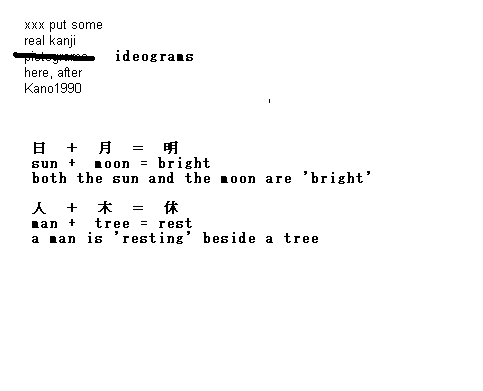
\includegraphics[scale=0.5]{images/kanjiideoograms.png}
\caption{Kanji ideograms}
\label{fig:kanjiideograms}
\end{figure}

\begin{table}[htbp]
  \begin{tabular}{| l c l |}
    \hline
    Class radical & Sound radical /ki/ & meaning \\
    \hline
    \cjk{土} ('earth') & \cjk{奇} & \cjk{埼} 'spit, promotory, cape' \\
    \cjk{山} ('mountain') & \cjk{奇} & \cjk{崎} 'promontory, cape, spit' \\
    \cjk{石} ('stone') & \cjk{奇} & \cjk{碕} 'cape, promontory, spit' \\
    \cjk{王} ('jade') & \cjk{奇} & \cjk{琦} 'gem, precious stone' \\
    \cjk{糸} ('thread') & \cjk{奇} & \cjk{綺} 'figured cloth, beautiful' \\
    \cjk{馬} ('horse') & \cjk{奇} & \cjk{騎} 'riding on horses' \\
    \cjk{宀} ('roof') & \cjk{奇} & \cjk{寄} 'to gather' \\
    \cjk{金} ('metal') & \cjk{奇} & \cjk{錡} 'cauldron, chisel' (Chinese only) \\
    \hline
  \end{tabular}
\caption{Kanji phonograms}
\label{table:kicombinations}
\end{table}

The Kanji can be classified according to their building principle:
\begin{enumerate}
 \item \textbf{Pictograms} are graphically simplified images of real artefacts.
       The examples in Fig~\ref{fig:kanjipictograms} 
       after~\shortciteANP{Kano1990}~\citeyear{Kano1990} show the graphical 
       reduction process. Pictograms are only a small minority among the Kanji,
       their number ranges around 120. Another 100 pictograms appear as a part of
       more complex characters~\shortcite{Foljanty1984}.
       
 \item \textbf{Ideograms} are combinations of two or more pictographical
       characters. They often bear a more abstract meaning than a simple 
       pictogram. The abstract meaning of the complex character is meant to be 
       associated with the content of the individual parts. The number of 
       ideograms is fairly small, too. Abstract terms like 
       'top' (Jap.~\cjk{上}, pron. \cjk{うえ}/ue), 
       'bottom' (Jap.~\cjk{下}, pron. \cjk{した}/shita),
       'left' (Jap.~\cjk{左}, pron. \cjk{ひだり}/hidari),
       'right' (Jap.~\cjk{右}, pron. \cjk{みぎ}/migi)
       and numbers like
       'one' (Jap.~\cjk{一}, pron. \cjk{いち}/ichi),
       'two' (Jap.~\cjk{二}, pron. \cjk{に}/ni),
       'three' (Jap.~\cjk{三}, pron. \cjk{さん}/san),
       'four' (Jap.~\cjk{四}, pron. \cjk{し}/shi),
       'five' (Jap.~\cjk{五}, pron. \cjk{ご}/go)
       and so forth can be regarded as parts of the 
       ideograms~\shortcite{Foljanty1984}.

 \item \textbf{Phonograms} are combinations of two Kanji characters. One of those
       refers to a concept class (for \emph{class characters} or \emph{radicals},
       see section~\ref{sec:radicals}), 
       while the other character exclusively bears a phonetic value. The content
       of the second part of a phonogram is not relevant and can be ignored.

       In table~\ref{table:kicombinations} the character 
       \cjk{奇} (Jap. pron. \cjk{き}/ki, Eng. 'strange') is used for the purpose
       of pronunciation only (/ki/), while the radical defines an
       object class. Object classes can be categories like 'human and human 
       actions', 'metal', 'horse', 'roof / under a roof' etc.
       The semantic identity within the \emph{Morphogram} is assembled with two
       reference figures. The pronunciation part is identical for all characters,
       it serves as a selection criterion within a semantic class selected by 
       the class radical~\shortcite{Foljanty1984}.

\end{enumerate}

As a character type, phonograms are predominant among the Hànzì. Therefore, the
phonogram concept, including the radical concept, was transferred to all Chinese 
characters. Pictograms that are class radicals themselves, are interpreted as 
characters with an empty sound radical. As the phonograms are historically the 
last development step of the Han characters, they constitute a different quality 
in the Chinese script. Phonograms mark the transition between a non-linguistic
pictographic script that does not represent linguistic units, but rather images 
of objects, to a linguistic script. In principle, there is no difference to
an alphbetical or syllabic script. Except, morphemes are represented instead of 
phonemes or syllables. However, one character often denotes more than one 
morpheme~\shortcite{Foljanty1984}.

In Japanese, basically the same relation between the Kanji characters and 
morphemes can be observed. However, the correspondence between the morphemes and 
the syllables (and thus the characters and syllables) is often missing.
Since Chinese has a monosyllabic morpheme structure, a one-to-one correspondence
between morpheme, character and syllable can be observed.
Congruence of character, morpheme and syllable in Japanese can only be found for
Chinese borrowings, but not all of them. The original Japanese vocabulary has
multisyllabic morphemes, therefore some impreciseness arises in the graphical
reproduction of the morpheme structure~\shortcite{Foljanty1984}.


\section{The Modern Japanese Writing System}
\label{sec:modernjapanesewritingsystem}

%xxx: see \shortcite{Foljanty1984} 3.1
%xxx: see \shortcite{Lange1922} p.64
%xxx: see \shortcite{Tsujimura2007} for morphology stuff
%xxx: see \shortcite{Grassmuck1997}





The Japanese writing system has a complex structure. The three scripts 
\emph{Hiragana} (sec~\ref{sec:hiragana}),
\emph{Katakana} (sec~\ref{sec:katakana}) and
\emph{Kanji} (sec~\ref{sec:compositionofkanji}),
are combined to one writing system. Each script has its task within the system:
\begin{itemize}

  \item Kanji are used to write lexical morphemes, i.e. content-bearing morphems.

  \item Katakana are used to transcribe foreign words, borrowings and 
        nonstandard areas.

  \item Hiragana are used to write grammatical morphemes and anything else that
        is not written in one of the other two scripts, e.g. the syllables
        of a word that has a Kanji character unknown to the writer.

\end{itemize}
The actual writing system is mainly based on Kanji and Hiragana, catenated to
Kanji-Kana blended writing.
\begin{exe}
\ex\label{mariaYamada}
\gll 
 \cjk{マリア:} 
 \cjk{山田さん、} 
 \cjk{「火の鳥」} 
 \cjk{という} 
 \cjk{アニメ} 
 \cjk{を} 
 \cjk{もう} 
 \cjk{見ました} 
 \cjk{か。} \\
% Maria: Yamada-San, [kanotori] toiu anime wo mou mimashita ka.\\
 Maria: Yamada-San, [Firebird] say anime \textsc{obj-particle} already seen \textsc{question-particle} \\
\trans 'Maria: Ms Yamada, say, have you seen the Firebird cartoon yet?' \\
Taken from~\shortcite{Katsuki2006Book}
\end{exe}
In example~(\ref{mariaYamada}), the blending of the different scripts 
can be seen:\\
Both the foreign name  \cjk{マリア} (Eng. 'Maria') and the borrowing 
\cjk{アニメ} (\emph{anime}, Jap. short for Eng. 'animation') are written in 
Katakana. Kanji are used for:
\begin{itemize}
\item The Japanese name \cjk{山田} (\emph{Yamada}).
\item The nouns \cjk{火}~(Eng. 'fire') and 
      \cjk{鳥}~(Eng. 'bird').
\item The verb stem \cjk{見}~(Eng. 'see').
\end{itemize}
The rest is written in Hiragana:
\begin{itemize}
  \item The politeness ending \cjk{さん}~(\emph{san}; 
        Eng. equiv. 'Mr/Ms/Mrs') for addressing a person with their name.
  \item The genitive particle \cjk{の}~(\emph{no}) between 
        \cjk{火}~(Eng. 'fire') and \cjk{鳥}~(Eng. 'bird'), to yield 
        \cjk{火の鳥}~(Eng. 'firebird').
  \item The interjection \cjk{とうい}~(Eng. 'say').
  \item The object particle \cjk{を}~(\emph{wo}).
  \item The adverb \cjk{もう}~(Eng. 'already').
  \item The past tense conjugation and politeness ending of the 
        verb \cjk{ました}~(\emph{mashita}).
  \item The question particle \cjk{か}~(\emph{ka}).
\end{itemize}

%\begin{CJK}
%マリア:山田さん、「火の鳥」 というアニメをもう見ましたか。
%\end{CJK}

Despite those complexities, other features of the Japanese writing system are 
simpler than in latin-based alphabetic scrips. 
For example, there is no capitals or lowercase letters.
Each character has a reserved space of roughly the same size.
In the following sections, the different scripts will be presented in greater 
detail.

\subsection{Kana \cjk{かな}}
\label{sec:kana}

If the Japanese had abolished the Chinese characters after formation of the
syllabic scripts and used only those, studying the Japanese script would not
such a complex task. \shortcite{Lange1922} reports about attempts to remove
the Kanji from Japanese and use the Kana or even Latin script, so called
\cjk{ロマジ} (\emph{romaji} Latin ('Roman') transcription of Japanese; Eng. lit.
'Roman characters'). However, non of those attempts succeeded and both Kana
scripts serve as auxiliary scripts. The \cjk{送り仮名}~(Jap. pron. \cjk{ オクリガナ}/okurigana; Eng. 'accompanying characters') are Hiragana that form a word 
together with a Kanji character.



xxx: see \shortcite{Foljanty1984} 2.2


\subsubsection{Hiragana \cjk{ひらがな}}
\label{sec:hiragana}

\subsubsection{Katakana \cjk{カタカナ}}
\label{sec:katakana}

\subsection{Composition of the Kanji \cjk{漢字}}
\label{sec:compositionofkanji}

xxx: see \shortcite{Lange1922} p.64

%xxx: Kurze erwaehnung der morphologie. Hiragana an verben zur konjugation. zusammenhang verben / nomen in kanji, 

\subsubsection{Graphemic Elements}
\label{sec:graphemicelements}

xxx: see \shortcite{Foljanty1984} 2.1.4.2

\subsubsection{Radicals}
\label{sec:radicals}

%xxx: see \url{http://japanese.about.com/library/weekly/aa070101a.htm} : radicals
%xxx: see \shortcite{Foljanty1984} 2.1.5 and 2.1.4
%xxx: see \shortcite{Lange1922} p.85ff p.94ff

\subsubsection{Readings}
\label{sec:readings}
Foljanty 2.1.7

\subsection{Structure of the Japanese Writing System}
\label{sec:structureofwritingsystem}
Having demonstrated the Hiragana in~\ref{sec:hiragana}, the Katakana 
in~\ref{sec:katakana} and the Kanji in section~\ref{sec:compositionofkanji}, 
it is now possible to report about the structure of the writing system as such.

%xxx: see \shortcite{Foljanty1984} 3.1-3.2
%xxx wird das nach einleitung ueberhaupt noch gebraucht?

\subsection{Romaji \cjk{ロマジ}}
\label{sec:romaji}
xxx: see \shortcite{Foljanty1984} 4

\subsection{Machine Writing of Japanese}
\label{sec:machinewritingofjapanese}

Machine processing of the Japanese scripts has been an issue, ever since humans
started to automate their writing.

xxx: see \shortcite{Lange1922} p. XII Stichwort Drucklegung
xxx: see \shortcite{Foljanty1984} 5
xxx: see MS IME dsecription (technical report or something?!)
xxx: see section \ref{sec:hwrofhanziandkanji} for a description of research 
efforts in order to provide technology for using handwriting as an input method 
for Japanese.
xxx: see \shortcite{Grassmuck1997}


\section{Difficulties of Writing Japanese for Learners}
\label{sec:writingjapanesedifficulties}


xxx: find places for citations of the following paper (if not already done)
\shortcite{Foljanty1984}
\shortcite{Lange1922}
\shortcite{Katsuki2006Book}
\shortcite{Katsuki2006Workbook}
\shortcite{Haschke2008}
\shortcite{Tsujimura2007}
\shortcite{Grassmuck1997}
